
%% Formato para la presentaci\'on de  proyectos de grado. 
%% Maestría en Ingeniería de Software
%% Pontificia Universidad Javeriana
%% Elaborado por Angela Villota y Luisa Rincón
%% Inspirado en Formato elaborado para carrera de Ing de Sistemas
%% V 1.0 Abril - 2022

\documentclass[12pt]{article}
\usepackage[utf8]{inputenc}
\usepackage{geometry}
\geometry{letterpaper}
\usepackage[spanish,es-tabla]{babel}
\usepackage{cite}
\usepackage{titling}
\usepackage{setspace}
\usepackage{graphicx}
\graphicspath{{img/}} %ruta de la carpeta en donde estaràn las imágenes
\usepackage{blindtext}
\usepackage{hyperref}
\usepackage{natbib} %% para citaciones
\usepackage[format=hang,font=small,labelfont=bf]{caption}

% *** ALIGNMENT PACKAGES ***
%
\usepackage{array}
\usepackage{booktabs}
\usepackage{pdflscape}
\usepackage{multirow}
\usepackage{float}
\usepackage{longtable}
\usepackage{dblfloatfix}
\usepackage{subfig}

\onehalfspacing
\setcounter{secnumdepth}{5}
\setcounter{tocdepth}{2}

\usepackage{xcolor}
\definecolor{light-gray}{gray}{0.95}
\newcommand{\code}[1]{\colorbox{light-gray}{\texttt{#1}}}

\renewcommand\maketitlehooka{\null\mbox{}\vfill}
\renewcommand\maketitlehookd{\vfill\null}


\begin{document}
%crear titulo
%\maketitle

%%%%%%%%%%%%%%%%%
% Portada del Anteproyecto
%%%%%%%%%%%%%%%%%
\begin{center}
\thispagestyle{empty}
\vspace*{0cm}
\begin{center}
    
\includegraphics[width=9cm]{pujlogo}~\\[1.75cm]
\end{center}
\textbf{\huge
Implementación de un proceso de integración continua para la ejecución de pruebas con alta cobertura y feedback oportuno}\\[1.75cm]
\Large\textbf{Andrés Felipe Burbano Castillo}\\[1.5cm]
\small Anteproyecto presentada(o) como requisito parcial para optar al
t\'{\i}tulo de:\\
\textbf{Magister en Ingenier\'{\i}a de Software}\\[1.5cm]
Director(a):\\
T\'{\i}tulo (Ph.D., MSc) Jaime Alberto Chavarriaga Lozano\\[1.6cm]

Pontificia Universidad Javeriana Cali\\
Facultad de Ingeniería\\
Departamento de Electrónica y Ciencias de la Computación\\
Cali, Colombia\\
\today\\
\end{center}

\newpage
%%%%%%%%%%%%%%%%%
% Ficha resumen
%%%%%%%%%%%%%%%%%
\thispagestyle{empty}
\begin{center}
    \Large{Ficha Resumen \\ Anteproyecto de Trabajo de Grado}
\end{center}

\textbf{Posible Título:}
\begin{enumerate}
    \item Área de trabajo:
    \item Tipo de proyecto (Aplicado, Innovación, Investigación):
    \item Estudiante:
    \item Correo electrónico:
    \item Dirección y teléfono:
    \item Director:
    \item Vinculación del director:
    \item Correo electrónico del director:
    \item Co-Director (Si aplica):
    \item Grupo o empresa que lo avala (Si aplica):
    \item Otros grupos o empresas:
    \item Palabras clave(al menos 5):
    \item Fecha de inicio:
    \item Duración estimada (en meses):
    \item Resumen:  Debe contener el tema a trabajar en el proyecto de grado, su importancia, la problemática que aborda, los objetivos propuestos, resultados esperado y posibles aplicaciones.  Debe ser redactado en un solo párrafo y no contener espacios entre líneas ni sangría.  Debe ser escrito con máximo 400 palabras 
\end{enumerate}

\newpage

%%%%%%%%%%%%%%%%%
% Indices y tablas
%%%%%%%%%%%%%%%%%

\tableofcontents
\listoffigures
\listoftables
\newpage

%%%%%%%%%%%%%%%%%
% Resumen / abstract
%%%%%%%%%%%%%%%%%
%%%%%%%%%%%%%%%%
% ABSTRACT
%%%%%%%%%%%%%%%%

\section*{Resumen}
Resumen en Inglés
150 palabras aprox

Esimula la capaidad de síntesis del autor. Puede ser más fácil de escribir al finalizar el anteproyecto pues en este punto el autor tiene mejor comprensión de su propuesta y del alcance que está tiene. 

No incluye citas o referencias bibliográficas.


\paragraph*{}{\textbf{Palabras Clave}}
Automatización de pruebas, Arquitectura de pipelines, Feedback oportuno, Reducción de bugs
\section*{Abstract}
Summary 
Around 150 words. 
\paragraph*{}{\textbf{Keywords}}
 
\newpage

%%%%%%%%%%%%%%%%%
% Introduccion
%%%%%%%%%%%%%%%%%
\section{Introducción}

Aquí algunos ejemplos de como se usan las imágenes, las tablas las listas

\textbf{ text in bold}
\textit{text in italics}
\underline{underlined text}
\texttt{text in consola-like font}

\subsection*{Ejemplos de listas}
itemize, enumerate, description

\begin{itemize}
    \item cada item es una viñeta
    \item Otra viñeta
\end{itemize}

\begin{enumerate}
    \item enumeración
    \begin{enumerate}
        \item anidado
    \end{enumerate}
\end{enumerate}

\begin{figure*}[htb]
\centering
\subfloat[] {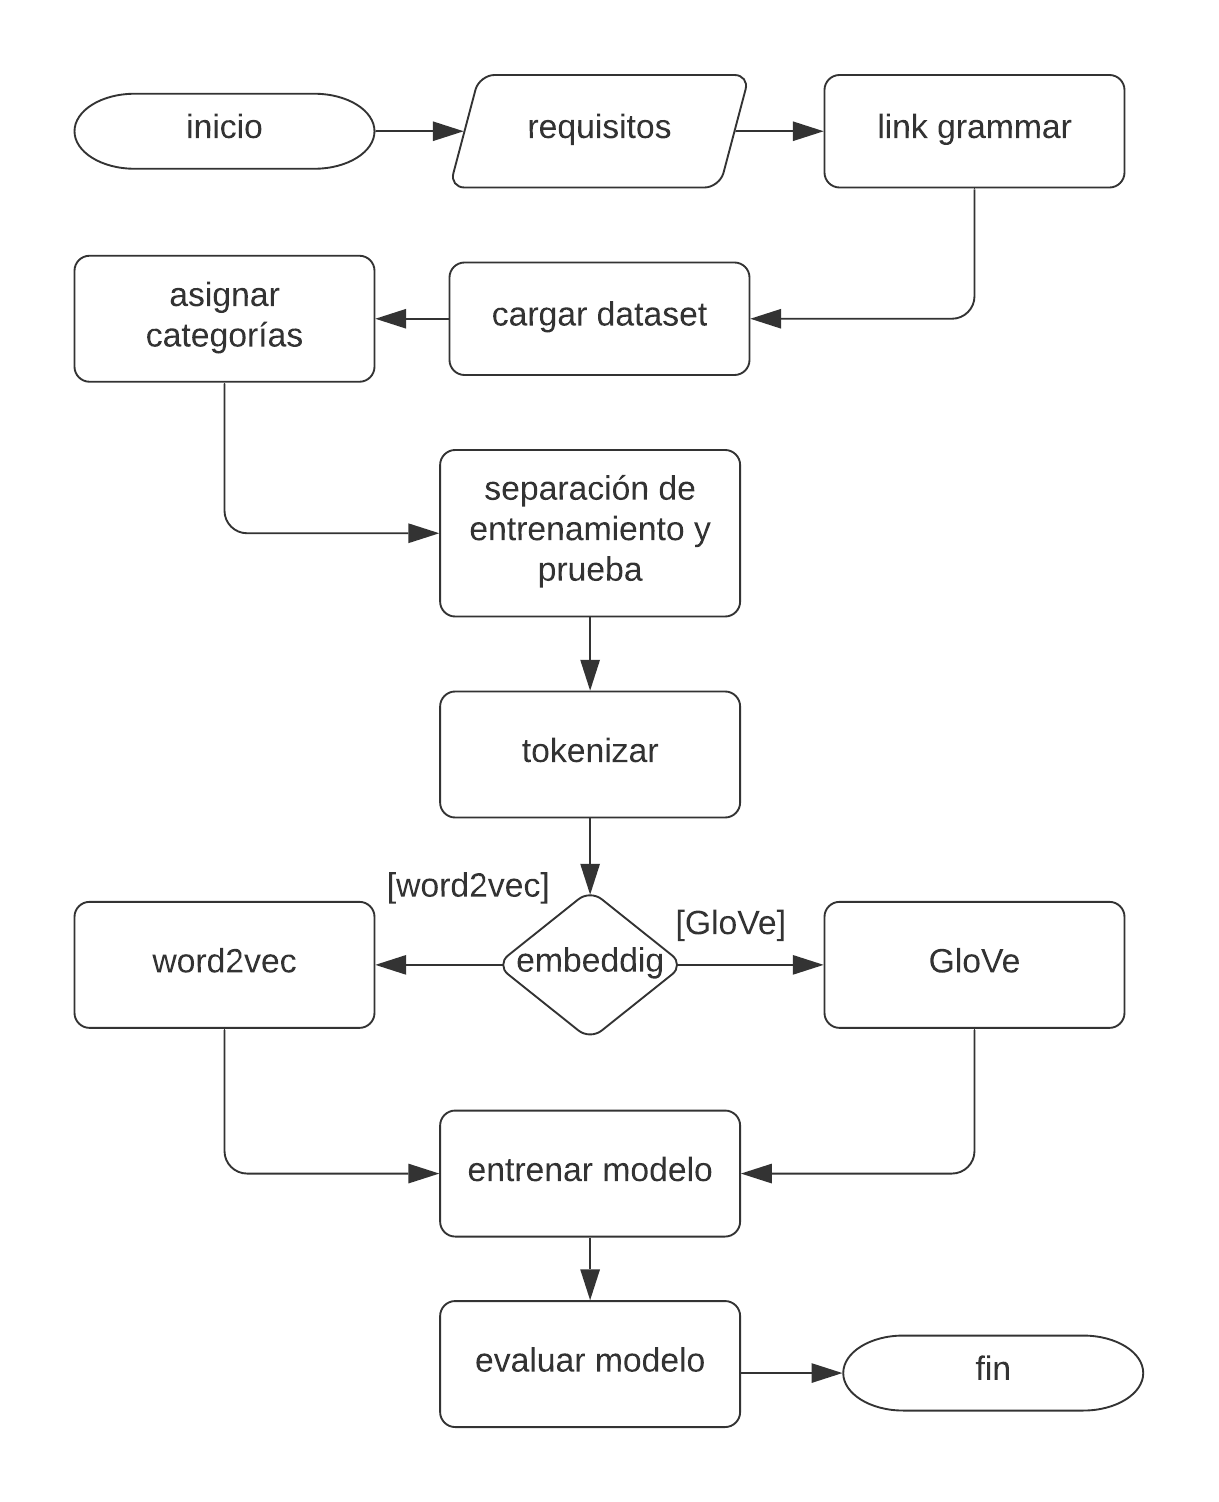
\includegraphics[width=0.5\textwidth]{Deep.png}

\label{fig:PAS_FM}}
\subfloat []{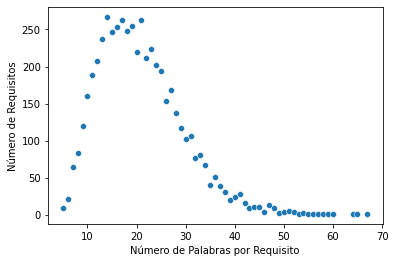
\includegraphics[width=0.38\textwidth]{freq_req.png}

\label{fig:PAS_FM2}}

\label{fig:examples}
\end{figure*}
 
 \begin{table}[htb]
     \centering
     \begin{tabular}{rc}
	\toprule
    	Item1 & Item2  \\
	\midrule
	celda 1 & celda 2\\
	\bottomrule

\end{tabular}
     \caption{Propuesta de elementos identificados en el desarrollo del proyecto. Fuente \citep{Hinton2012}}
     \label{tab:my_label}
 \end{table}

\subsection*{Uso de figuras}
La Figura \ref{fig:figure1} muestra un gráfico de ejemplo. Las tablas y figuras que aparecen en el documento deben ser previamente introducidas y explicadas


\begin{figure}
\centering
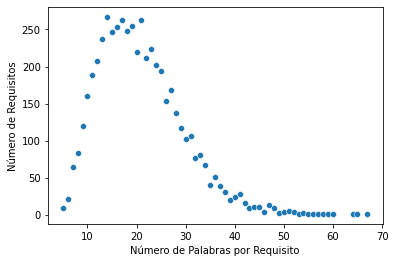
\includegraphics[width=0.5\textwidth]{freq_req.png}
\caption{Grafico tridimensional. Elaboración propia}
\label{fig:figure1}
\end{figure} 
\newpage

%% Problema
\section{DEFINICIÓN DEL PROBLEMA DE INVESTIGACIÓN}

\subsection{PLANTEAMIENTO DEL PROBLEMA}
Uno de los mayores desafíos que enfrentan las empresas es tener la capacidad de lanzar al mercado de manera frecuente software que sea innovador, seguros, con altos estándares de calidad que satisfagan las necesidades de sus usuarios. De lo contrario las empresas se exponen a pérdidas monetarias y de mercado, a daños reputacionales y sanciones por parte de los entes reguladores. Es por esto por lo que se contemplan diferentes metodologías, prácticas y técnicas para apalancar el proceso de desarrollo de software permitiendo así evaluar diferentes escenarios durante la construcción de las soluciones digitales. Una de estas técnicas es el aseguramiento de la calidad del software, ya que permite validar un buen y correcto funcionamiento del sistema desde condiciones normales hasta inusuales ayudando a mitigar los riesgos mencionados anteriormente.

Dentro del proceso de desarrollo de software se encuentra el proceso de Continuous Integrations por sus siglas en inglés (CI). Es una práctica del desarrollo de software, en donde los desarrolladores integran el código fuente con frecuencia y cada integración  es  verificada por un sistema que construye el código y lo prueba automáticamente \citep {martin} (Fowler, 2006). Las pruebas continuas o Continuous Testing  por sus siglas en inglés (CT), es un término introducido por Edward Smith en el año 2000 (Smith, 2000). Consistía  en  un  proceso de ejecución de pruebas durante todo el día (continuamente), mientras se desarrollaba el código. Sin embargo, este concepto ha ido evolucionando con el tiempo. En  el año 2010, este concepto se extiende a otros tipos de pruebas (Burgin, 2010): pruebas de especificación, pruebas de diseño, pruebas sobre el código  fuente,  pruebas funcionales,  pruebas no funcionales, pruebas de instalación, pruebas de soporte y pruebas de mantenimiento. El mayor problema que enfrentan los equipos de desarrollo de software  hoy en día es poder identificar qué tipo de prueba realizar y lograr obtener un feedback apropiado y oportuno de acuerdo a cada ejecución realizada con el objetivo de desplegar cambios que aporten valor continuamente en los diferentes ambientes como Desarrollo, Staging, Producción ya sea diario, semanal, quincenal o mensual, esto debido a que existen diferentes pruebas como son las unitarias, las de componente, de integración y regresión donde cada una de estas tienen diferentes enfoques de aplicación y su retroalimentación varía en cada caso de acuerdo a su frecuencia de despliegue.

Las pruebas unitarias que aplique el equipo de desarrollo no tienen la cobertura necesaria para asegurar la calidad del software puesto no cubre todas las casuísticas del negocio, el feedback que el equipo de desarrollo puede tener por parte de QA puede llegar a tomar días dado que se debe realizar un análisis previo puesto que la comunicación entre QA y Desarrollo no es directa, el equipo de desarrollo no tiene claro que tipo de prueba aplicar de acuerdo a cada funcionalidad generando un vacío en el proceso de desarrollo al momento de realizar un despliegue, los tiempo de ejecución de pruebas pueden tardar días dado que no se tiene automatizado flujos críticos de negocio.

Las causas mencionadas anteriormente denotan que si no hay una comunicación  asertiva rápida y eficaz sobre el resultado del proceso de pruebas o testing genera retrasos en las fechas pactas y sobre costos en el proyecto puesto que no se tiene una estrategia clara durante el proceso de desarrollo de software y se desconoce sobre las herramientas y procesos que permitan al equipo de desarrollo realizar una integración continua junto con QA enfocado a pruebas para desplegar cambios que generen valor al usuario. La calidad debe estar a cargo de todo el equipo de trabajo por ende se puede llegar a tener bugs que se pudieron mitigar previamente y esto conlleva a que estos bugs puedan salir en producción generando los riesgos mencionados al inicio.

\subsection{FORMULACIÓN DEL PROBLEMA}
De acuerdo al planteamiento del problema, se realiza la siguiente formulación:

¿Cómo identificar los diferentes tipos de pruebas que se deben realizar?
¿Cómo implementar un set de pruebas para cada despliegue?
¿Cada cuanto se deben ejecutar las diferente pruebas de acuerdo a cada despliegue?
¿Cómo obtener un feedback personalizado de acuerdo a cada ejecución de pruebas?
¿Cómo implementar una arquitectura de pipelines para la ejecución de pruebas para los diferentes despliegues con feedback inmediato bajo el modelo CIVIT?

\newpage

%% Objetivos
\section{Objetivos del proyecto}
Los objetivos deben formularse de manera que logren transmitir lo que intenta realizar el investigador y lo que espera obtener como resultado. 

Los objetivos deben iniciar con un verbo en infinitivo (construir, diseñar, seleccionar, analizar, modelar simular, etcétera.) 




\subsection{Objetivo General}
Este objetivo evidencia lo que se quiere lograr en la investigación. Suele estar ligado a la pregunta de investigación definida en el planteamiento del problema pues relaciona ante el problema de investigación qué quiero hacer o qué hará el estudio ha abordar.

En resumen el objetivo general responde \textbf{¿qué se espera lograr con el proyecto de grado?}


\subsection{Objetivos específicos}
Señalan los aspectos que dentro del objetivo general serán objeto de especial atención por parte del investigador. Por lo general cada objetivo específico corresponde a una etapa de la investigación pues son los logros parciales que el investigador espera cumplir y que, en su conjunto, permiten alcanzar el objetivo general. \\

La suma de los objetivos específicos equivaldría al objetivo general. Los objetivos definen los compromisos que se adquieren por parte del investigador al desarrollar el proyecto.  


\subsubsection*{Errores en la formulación de objetivos}

\textbf{Englobar varios objetivos en un solo enunciado.} Esto ocurre cuando no se tiene claro cuáles son los ejes de investigación del proyecto.



\textbf{Formular objetivos fuera del alcance.} Los objetivos se deben alcanzar en el tiempo establecido para la investigación, con los recursos disponibles para el o los investigadores.La lista de objetivos sirve a los evaluadores para determinar el alcance y el logro de cada uno de ellos. 

\textbf{Definir activades no objetivos.} Los objetivos deben lograrse, los pasos de la metodología sólo deben realizarse o ejecutarse. Por esta razón es posible que uno o más pasos metodológicos deben ejecutarse dos o más veces antes de lograr que un objetivo específico se declare como logrado. Por ejemplo: \textit{diseñar encuesta de satisfacción} es una actividad,  mientras que \textit{evaluar la solución propuesta en términos de la percepción de utilidad y la intención de uso} es un objetivo. 




\subsection{Resultados esperados}
Los resultados esperados se redactan teniendo en cuenta los objetivos de investigación, el problema que se quiere investigar, y las posibilidades reales de producir los mismos reconociendo las condiciones en que puede operarse o ejecutarse el proyecto de investigación.
\newpage

%% Alcance
\section{Alcance}
Se analiza cada objetivo específico, buscando delimitar con mayor precisión qué se va a hacer y qué no.
Deja claras limitaciones ya identificadas en la solución que se va a construir.
Identifica algunos obstáculos que eventualmente pudieran presentarse durante el desarrollo de la investigación.
Define hasta dónde llegará el trabajo.

\newpage

%% Justificacion
\section{Justificación del trabajo de grado}
Este texto explica porque la solución contribuye a mejorar las condiciones adversas de los afectados en forma negativa por el problema. Explica ¿qué pasaría si SI se resuelve el problema de investigación?

Se suele redactar en términos de impactos, contribuciones positivas para generar nuevo conocimiento o experiencias. 

Explica qué beneficios genera la solución del problema, por ejemplo en lo económico, social, ambiental, etc a los afectados negativamente por el problema.

¿Qué impactos y beneficios genera la solución del problema, en lo económico, social, ambiental, etc.? 

\textbf{Nota:} Respalde las afiramaciones con evidencias y hechos verificables que hayan sido documentados a través de publicaciones científicas y/o ingeniería. 

\newpage

%% Marco conceptual
\section{Marco teórico de referencia y antecedentes}
Es una recopilación de información de todo aquello que se haya hecho alrededor del tema propuesto. Sirve como una orientación acerca del enfoque que debe darse al proyecto, porque al acudir a los antecedentes, el proponente puede darse cuenta de cómo ha sido tratado el problema: qué tipos de estudio se han efectuado sobre él, qué modelos y diseños se han utilizado, dónde y cómo se han recolectado los datos, etc. 

\textbf{La construcción del estado del arte sirve como punto de partida para la realización del proyecto.}

Para el anteproyecto se recomienda una extensión de máximo 10 páginas para esta sección.

\subsection{Bases Teóricas}
En esta sección se describen los fundamentos teóricos que sustentan el trabajo de investigación o proyecto de grado, con sus respectivas citas bibliográficas (Es muy importante el manejo riguroso de las citas). 

Tenga encuenta la siguiente lista de chequeo:
\begin{itemize}
    \item Los temas tratados en el marco teórico deben ser relevantes al problema que se está abordando. Estas descripciones no deben ser demasiado extensas ni repetir la teoría que está en los libros, debe presentar los conceptos fundamentales y hacer referencias a libros o artículos donde esos temas se tratan con mayor detalle. 
    \item Los temas aquí abordados deben ser relevantes con el fin de hacer el documento autocontenido.
    \item NO asuma que el lector es un experto 
    \item NO se trata de una enumeración de
fuentes y conceptos aislados, sino de que presenta de manera artículada los conceptos relevantes para entender la investigación. 
\item Use las definiciones de los autores "seminals" o los autores referentes del área. 
\end{itemize}

Tips de lo que no va:
\begin{itemize}
\item  NO incluir material que el lector no necesita para entender lo que sigue
\item  No incluya material que no se conecta con alguna sección de la tesis
\item NO incluya temas que rompan el flujo del argumento. Algunas cosas pueden parecer importantes pero podrían ser Anexos. 
\end{itemize}

\subsection{Estado del Arte}
Esta sección da cuenta del estado en el que se encuentra la investigación sobre el tema que se está explorando con el proyecto de grado. Tiene como objetivo revisar y analizar el conocimiento acumulado alrededor del problema, y evidenciar cuál es el estado actual de la solución a un problema respecto al problema que se desea abordar. 

Esta sección presenta trabajos previos (estudios o implementaciones) que abordan el problema de forma similar, da confianza sobre el conocimiento del autor de referentes anteriores así como permite que no se repitan estudios sobre asuntos explorados previamente.

\textbf{Nota:} \textit{En el anteproyecto este análisis puede ser más superficial pero a medida que lo haga mejor podrá reutilizar más para su documento final.}

\subsubsection*{¿Qué incluir?}
Piense en los siguientes temas:
\begin{itemize}
    \item ¿Cómo se ha resuelto el problema?
    \item ¿Quienes han resuelto el problema?
    \item ¿Qué aspectos técnicos económicos, culturales normativas estándares se han tenido en cuenta?
    \item ¿El problema ha sido resuelto en otro contexto?
\end{itemize}

\subsubsection*{¿Qué NO debe incluir?}
\begin{itemize}
    \item NO incluya ideas propias o reflexiones respecto a cómo solucionar el problema. Facts only. 
    \item NO describa información de otros trabajos o problemáticas que usted NO va a abordar 
\end{itemize}

\subsubsection*{¿Cómo organizarlo?}
\begin{itemize}
    \item Definición de un conjunto de criterios que van a usarse para comparar los trabajos de otros
    \item Una descripción corta de cada propuesta - previas de solución del problema. Resalte en cada una ventajas y desventajas. 
    \item  Indique de forma clara: ¿Por qué las propuestas y soluciones revisadas no sirven en el contexto del estudio y porque no resuelven la pregunta planteada en su proyecto de investigación?
    \item \textbf{DESEABLE}: haga tablas o gráficas que presenten cuál es el vacío que tiene la situación actual. 
\end{itemize}



\newpage

%% Metodología
\section{Metodología de la investigación}
La metodología debe reflejar la estructura lógica del proceso de investigación. Esta sección define y explica la selección de la estrategia adoptada para responder al problema planteado y además explica el cómo va a realizar la investiga. 

La metodología indica cómo será el proceso desde la recolección de los datos, la organización, sistematización, y análisis de la información, hasta la forma como se van a interpretar y presentar los resultados.   Si bien esto puede cambiar en la realización del proyecto una metodología concreta permite tener una guía para la elaboración del proyecto. 

La metodología definida debe reflejar la articulación entre los objetivos, el proyecto y los procedimientos para cumplir dichos objetivos. 


\newpage

%% Recursos
\section{Recursos a emplear}
Esta sección resume los recursos que van a emplearse en el desarrollo del proyecto de grado. Los recursos que deben considerarse incluyen a las personas que estarán involucradas en el proyecto y a los materiales como licencias, libros, etc.  A continuación se listan los posibles recursos que se requieren en un proyecto de grado.
\begin{enumerate}
    \item Recursos Humanos
    \begin{enumerate}
        \item Director
        \item Co-Director (si existe)
        \item Asesor (si existe)
        \item Grupo de Investigación de la Facultad que lo avala
        \item Otros grupos
    \end{enumerate}
    \item Económicos
    Presupuesto General de recursos requeridos (materiales, insumos, equipos, software y material bibliográfico)
\end{enumerate}
\newpage

%% Cronograma
\section{Cronograma de actividades}
\newpage

\section{Referencias Bibliográficas}
Se deben presentar de forma rigurosa y completa las referencias bibliográficas utilizadas en el documento (No incluir bibliografía no referenciada en el documento). Se debe seguir una sola norma de referenciación en todo el documento, ej. IEEE, Harvard o APA.

Utilizar en lo posible bibliografía reciente de fuentes confiables y en inglés(libros, artículos científicos, etc.). Evitar utilizar fuentes no confiables como blogs, Wikipedia, o documentos sin autor.
%\bibliographystyle{IEEEtran}
\bibliographystyle{apalike}
\bibliography{bibfile}
\newpage

\section{Glosario de Términos}
Esta sección presenta un conjunto de definiciones cortas de términos que se usan en el documento del proyecto.  A continuación se presenta un extracto de un glosario de términos tomado de la tesis de ...

\begin{description}
\item[Accuracy] Métrica del porcentaje de clasificaciones correctas de un modelo de
aprendizaje supervisado.
\item[Bootstrap] En el contexto del aprendizaje de conjuntos de hipótesis,
es el uso de un subconjunto aleatorio de atributos y datos de entrenamiento obtenido
a partir de los datos originales, con esto se espera reducir la posibilidad de
\emph{overfitting}.
\item[Corpus] Un corpus lingüistico es un conjunto amplio de ejemplos reales del uso de un
lenguaje.

\end{description}





\end{document}
